\section{The algorithms}
\label{sec:algorithms}

Three algorithm families carry the whole behaviour: Artificial Potential
Fields (goal seeking and inter-robot spacing), the VFH family (obstacle
avoidance --- deterministic, predictive, and the probabilistic P-VFH proposal
of Section~\ref{sec:pvfh}), and the rigid-transport frame logic that ties the
four robots into one body. They compose into the steering-law variants
compared in Section~\ref{sec:fourvariants}, alongside two external
baselines (Follow-the-Gap, a Dynamic-Window planner and a
receding-horizon MPC, \S\ref{sec:baselines}).

\subsection{Artificial Potential Fields (APF)}

\code{apf\_force.m} computes an unnormalised force as the sum of a conic
attraction and a linear inter-robot repulsion:
%
\begin{align}
\mathbf{F}_{\mathrm{att}} &= w_{\mathrm{att}}\,
\frac{\mathbf{g} - \mathbf{p}}{\lVert \mathbf{g} - \mathbf{p} \rvert}, \\[4pt]
\mathbf{F}_{\mathrm{rep}} &= w_{\mathrm{rep}} \sum_{j \,:\, d_{ij} < d_0}
(d_0 - d_{ij})\, \frac{\mathbf{p} - \mathbf{p}_j}{d_{ij}}, \\[4pt]
\mathbf{F} &= \mathbf{F}_{\mathrm{att}} + \mathbf{F}_{\mathrm{rep}} .
\end{align}
%
Design choices that matter:

\begin{itemize}[leftmargin=1.6em]
\item \textbf{Conic (constant-magnitude) attraction}, not a quadratic well. A
quadratic field makes the robot crawl to a stop far from the goal; here the
approach slowdown is handled explicitly by the caller
($v \propto \min(1, e/r_{\mathrm{slow}})$), so the field itself stays sharp.
\item \textbf{Linear-in-gap repulsion}, exactly zero at $d = d_0$: no force
discontinuity at the boundary of the influence region, hence no chatter when
a neighbour sits at the edge of range.
\item \textbf{Obstacle avoidance is deliberately absent.} APF repulsion from
two nearby obstacle faces can cancel, leaving zero usable gradient --- the
classical local-minimum trap. All obstacle work is done by VFH.
\end{itemize}

\subsection{p-VFH: polar histogram obstacle avoidance}

\code{pvfh\_scan.m} consumes a \emph{LaserScan} (exactly what a ROS~2 node
reads off \code{/scan}), not a point cloud. Pipeline:

\begin{enumerate}[leftmargin=1.9em]
\item \textbf{Sense.} Analytic raycast, $n_{\mathrm{beams}} = 288$ over
$(-\pi, \pi]$ (open interval --- no duplicated beam at the seam), range
$d_{\mathrm{sense}} = 4.0 + \text{margin}$.
\item \textbf{Polar obstacle density.} $S = 72$ sectors; each sector takes the
\emph{nearest} hit along its bearing and accumulates
$h(s) = \exp(-d^2 / 2\sigma^2)$, with
$\sigma$ \emph{derived} from the required clearance:
$\sigma = (r_{\mathrm{eff}} + g_{\mathrm{react}})\,/\,\sqrt{2\ln(1/\tau)}$.
A fixed $\sigma$ silently hard-codes a fixed reaction distance; deriving it
keeps the reaction margin at $g_{\mathrm{react}} = 1.0$~m beyond the body
whatever the body size.
\item \textbf{VFH+ enlargement.} A hit at range $d$ blocks every bearing
within $\gamma = \arcsin(r_{\mathrm{eff}}/d)$ of it --- a body of effective
radius $r_{\mathrm{eff}}$ steered down any of those bearings would still clip
the obstacle. $r_{\mathrm{eff}}$ is the formation circumradius plus the robot
radius, i.e.\ the histogram is built \emph{for the whole payload}, not the
centre point.
\item \textbf{Circular smoothing.} Window 5 over the polar histogram with
wrap-around at $\pm\pi$ (smoothing it as a line segment leaves a seam
directly behind the robot --- a real bug that produced unexplained turns).
\item \textbf{Valley selection.} Candidate sectors with $h < \tau = 0.3$,
restricted to $\pm 45^\circ$ of the goal bearing; cost
$\lvert \operatorname{wrap}(s - \theta_{\mathrm{goal}})\rvert
+ 0.6\,\lvert \operatorname{wrap}(s - \theta_{\mathrm{prev}})\rvert$ (goal
alignment + heading hysteresis).
\item \textbf{Close-range reflex.} A repulsive term straight off the scan for
everything inside $d_{\mathrm{danger}} = 1.2 + \text{margin}$, weighted
$1/d^3$ and integrated over bearing (so the magnitude is resolution-independent).
\end{enumerate}

\subsection{The steering-law comparison}
\label{sec:fourvariants}

The paper's central experiment compares \textbf{eight steering laws} that all
consume a scan from the \emph{same front end} (\code{scan\_ranges\_dyn} $+$
\code{sensor\_noise}, Section~\ref{sec:sensornoise}): the same beam fan, the
same noise model, the same seeded random stream. The axis is selected by
\code{cfg.algo} and dispatched by \code{steering\_dispatch.m}:

\begin{table}[h]
\centering
\small
\begin{tabular}{@{}llp{4.4cm}l@{}}
\toprule
\code{cfg.algo} & Steering law & Occupancy / decision & Mover horizon\\
\midrule
\code{'apf'} & APF reflex only & --- (no histogram) & none\\
\code{'vfh'} & deterministic VFH+ & $\mathrm{env}(d_{\mathrm{meas}})$ & none\\
\code{'fgm'} & Follow-the-Gap & widest free arc & $T_{\mathrm{lead}}$\\
\code{'dwa'} & Dynamic-Window arcs & arc clearance $+$ heading & $T_{\mathrm{lead}}$\\
\code{'mpc'} & receding-horizon MPC & optimised turn-rate sequence & $T_{\mathrm{lead}}$\\
\code{'pvfh'} & predictive VFH+ & $\mathrm{env}(d_{\mathrm{meas}})$ & $T_{\mathrm{lead}}$\\
\code{'pvfh\_filt'} & pVFH $+$ range filter (ablation) & $\mathrm{env}(\hat d)$ on filtered ranges & $T_{\mathrm{lead}}$\\
\code{'pvfh\_prob'} & \textbf{P-VFH (proposal)} & $u_b$ on filtered ranges, eq.~\eqref{eq:ukernel} & $T_{\mathrm{lead}}$\\
\bottomrule
\end{tabular}
\caption{The comparison axis. ``Mover horizon: none'' means the scan shows
each mover where it is \emph{now}; $T_{\mathrm{lead}}$ means the scan also
carries the movers' contracted poses over the next $0.5$~s.}
\label{tab:algos}
\end{table}

The four histogram laws form an \textbf{ablation ladder}, each step
changing one thing: \code{'vfh'} $\to$ \code{'pvfh'} adds the mover
prediction horizon; \code{'pvfh'} $\to$ \code{'pvfh\_filt'} adds the
recursive range filter of \S\ref{sec:rfilter}; \code{'pvfh\_filt'} $\to$
\code{'pvfh\_prob'} replaces the deterministic occupancy by its posterior
expectation. The paired analysis of \S\ref{sec:paired} reports each step.
The external baselines get the same mover horizon as the proposal, so the
comparison with them is about the steering law and not about who was told
where the movers are going.

\paragraph{Corrected in the October 2026 audit.} Before the audit this table
did not describe the code: \code{'pvfh'} raycast a \emph{noise-free} lidar
and ignored the sensor model (so it was identical across seeds), and
\code{'vfh'} silently inherited the prediction horizon. Both now do what the
table says (\S\ref{sec:audit}).

\subsection{External baselines: Follow-the-Gap, Dynamic-Window, receding-horizon MPC}
\label{sec:baselines}

A comparison confined to one algorithm family invites the obvious question
of how an off-the-shelf local planner does on the same input. Three standard
local planners are therefore implemented at the \emph{same interface}
(same scan, same body radius, same blend with the goal attraction, same
speed and safety-gate logic):

\begin{itemize}[leftmargin=1.6em]
\item \textbf{Follow-the-Gap} (\code{'fgm'}, Sezer and G\"okasan
\cite{sezer2012}). Every return closer than the reaction envelope
$d_{\mathrm{block}}$ is an obstacle and blocks the bearings within
$\arcsin(r_{\mathrm{eff}}/d)$ of it; the widest run of free beams is the
gap, with centre $\phi_{\mathrm{gap}}$; the commanded heading is the
weighted mean
$\phi = \bigl(\tfrac{\alpha}{d_{\min}}\phi_{\mathrm{gap}} +
\phi_{\mathrm{goal}}\bigr)/\bigl(\tfrac{\alpha}{d_{\min}} + 1\bigr)$,
$\alpha = 2$~m, so the gap centre dominates as the nearest obstacle closes.
\item \textbf{Dynamic-Window arcs} (\code{'dwa'}, Fox, Burgard and Thrun
\cite{fox1997}). Candidate arcs $(V, \omega)$, $\omega \in [-1.5, 1.5]$
rad/s in 31 samples, are rolled out for $2$~s against the obstacle points
of the scan; arcs on which a body of radius $r_{\mathrm{eff}}$ touches a
point within $1$~s are inadmissible; the survivor maximising
$0.8\,\mathrm{heading} + 0.2\,\mathrm{clearance}$ wins.
\item \textbf{Receding-horizon MPC} (\code{'mpc'}): the
trajectory-optimisation class of local planner (the family of TEB, MPC and
MPPI \cite{rosmann2017,williams2017}) reduced to its core. Every step it
optimises a \emph{sequence} of three turn-rate segments ($0.8$~s each,
five levels in $[-1.2, 1.2]$~rad/s, so $125$ candidate sequences over a
$2.4$~s horizon) against the obstacle points of the scan, applies the first
move and re-plans. Cost: negative progress toward the goal, plus a soft
barrier $\max(0, 0.5 - \mathrm{clearance})^2$ averaged over the horizon,
plus small penalties on turn rate and on its changes; hard constraint: the
body stays clear for the first second. Unlike the Dynamic-Window planner
(one constant arc) a sequence can plan an S-manoeuvre. The search is an
exhaustive lattice rather than random shooting, so the planner draws no
random numbers and the seeded design of the study is preserved.
\end{itemize}

\paragraph{What these baselines are and are not.} They are faithful to the
published decision rules but adapted to this mission's interface: the
mission layer owns the speed (constant $V$ with the mover slowdown), so the
Dynamic-Window and MPC searches are over turn rate only. The MPC is a
compact representative of its class, not the TEB or MPPI implementation of
a navigation stack (no time-elastic band, no continuous optimiser, a
coarse lattice); none of the three is a tuned production planner. Their
parameters were set once and not tuned against the results.

\subsection{Sensor noise: one model for every variant}
\label{sec:sensornoise}

\code{sensor\_noise.m} is the single noise model consumed by all four
variants, so the comparison isolates the steering law (the same contract the
ROS~2 port keeps in \code{vfh.py::sensor\_noise}). Two modes:

\begin{itemize}[leftmargin=1.6em]
\item \textbf{\code{'lidar'}} --- dense $360^\circ$ scan, homoscedastic
Gaussian noise: $d_{\mathrm{meas}} = d + \mathcal{N}(0, \sigma_0^2)$ with
$\sigma_0 = 0.02$~m.
\item \textbf{\code{'tof'}} --- sparse direct-ToF array (VL53L1X/
VL53L5CX-class): beams cover a limited field of view
($\code{fov\_deg} = 60^\circ$, centred on the \emph{body heading} --- the fan
is mounted on the payload and turns with it) and
every range carries \emph{distance-dependent} noise
$\sigma(d) = \sigma_0 + k_{\mathrm{rng}}\,d$ with $k_{\mathrm{rng}} = 0.03$,
the standard error model for direct time-of-flight ranging (sigma grows with
range and with target-reflectivity loss).
\end{itemize}

Both modes apply a \textbf{max-range drop-cut}: a (noisy) return at or beyond
\code{max\_range} reports \code{max\_range}, reproducing the real edge
behaviour where a weak far return is indistinguishable from no return.
Consumers treat max-range returns with reduced confidence: P-VFH floors their
blocked probability at $p_{\mathrm{unknown}} = 0.05$.

\subsection{P-VFH: the probabilistic histogram (the proposal)}
\label{sec:pvfh}

\code{pvfh\_prob.m} replaces the deterministic occupancy value of the
histogram with a probabilistic one, keeping the entire control topology
(VFH+ enlargement, threshold, valley search, hysteresis, APF reflex fusion)
identical. The motivation: thresholding a \emph{graded kernel of the measured
range} is brittle under noise in two opposite directions --- a return
measurably inside the reaction envelope can still leave the corridor reading
``free'' (missed obstacle), while a single low noise outlier seals a corridor
the deterministic stack would have used (spurious blocking).

\paragraph{Per-beam risk.} Model the measurement as
$d_{\mathrm{meas}} = d + e$, $e \sim \mathcal{N}(0, s_b^2)$ with $s_b$ the
per-beam sigma of Section~\ref{sec:sensornoise}; the true range $d$ is the
unknown. The physics is one-sided --- the beam stopped where it stopped, so
there is nothing behind the return --- hence the blockage belief lives on
$d \in (0, d_{\mathrm{meas}}]$:
\begin{equation}
p_b \;=\; P\bigl(d \le d_{\mathrm{block}} \mid d_{\mathrm{meas}}\bigr)
\;=\; \Phi\!\Bigl(\frac{d_{\mathrm{block}} - d_{\mathrm{meas}}}{s_b}\Bigr),
\qquad d_{\mathrm{block}} = r_{\mathrm{eff}} + g_{\mathrm{react}}.
\label{eq:prise}
\end{equation}
The $p = 0.5$ crossing sits exactly at $d_{\mathrm{meas}} = d_{\mathrm{block}}$
--- the same reaction envelope the deterministic \code{auto\_sigma} contract
encodes --- and the transition width is the sensor's own uncertainty: no
hand-tuned safety inflation. Per sector the $p_b$ are pooled with a
\textbf{noisy-OR}, the correct combiner for independent chances of the same
fatal event,
\begin{equation}
p_s = 1 - \prod_{b \in s} (1 - p_b),
\label{eq:noisyor}
\end{equation}
which reduces to $\max_b p_b$ for dense LiDAR (first hit wins; the rest are
occluded) and adds evidence for sparse ToF, where several beams genuinely
cover one sector. Unobserved sectors and drop-cut returns floor at
$p_{\mathrm{unknown}}$: absence of evidence is not evidence of absence.
\textbf{The risk layer is a diagnostic output}: $p_b$ and $p_s$ are computed
and logged, but --- for the reason in the next paragraph --- they do not
enter the steering decision. (Earlier text credited the noisy-OR pooling
with the sparse-sensor results; the code never used it for steering.)

\paragraph{Why the selection cannot threshold $p$.} A probability saturates:
any return measurably inside $d_{\mathrm{block}}$ gives $p_s \to 1$, so every
VFH+ enlarged arc becomes a full-amplitude plateau, circular smoothing then
seals even wide gaps between obstacle clusters, and the stack stalls. This
failure mode was reproduced, diagnosed sector-by-sector, and is the reason
the selection layer is not the risk layer.

\paragraph{The selection kernel.} The histogram is instead built from the
\textbf{posterior expectation of the deterministic kernel}
$\mathrm{env}(d) = e^{-d^2/2\sigma_h^2}$ (with $\sigma_h$ the same
\code{auto\_sigma} width as the deterministic stack) under the sensor
likelihood $d \sim \mathcal{N}(d_{\mathrm{meas}}, s_b^2)$, which has the
closed form
\begin{equation}
u_b \;=\; E\bigl[\mathrm{env}(d)\bigr]
\;=\; \sqrt{\frac{\sigma_h^2}{\sigma_h^2 + s_b^2}}\;
\exp\!\Bigl( -\frac{d_{\mathrm{meas}}^2}{2\,(\sigma_h^2 + s_b^2)} \Bigr).
\label{eq:ukernel}
\end{equation}
Three properties make this the right bridge between the probability layer and
the control law:
\begin{enumerate}[leftmargin=1.9em]
\item \textbf{Exact deterministic limit.} As $s_b \to 0$,
$u_b \to \mathrm{env}(d_{\mathrm{meas}})$: with a precise sensor P-VFH
\emph{is} the verified deterministic stack --- the low-noise behaviour is
inherited constructively, not re-tuned (unit-tested:
\code{test\_pvfh\_prob\_matches\_deterministic\_at\_low\_noise}).
\item \textbf{Bounded and graded.} $u_b < 1$ always; enlarged arcs carry
range-graded values, so valleys survive smoothing exactly as in the
deterministic stack.
\item \textbf{A reaction envelope that widens with noise.} The range at
which a return crosses the threshold grows with $s_b$
(Proposition~2): a noisier sensor makes the law react
earlier. This is the mechanism the noise ablation (Section~\ref{sec:e2})
tests.
\end{enumerate}

\paragraph{What the kernel alone does not do.} The properties below are
properties of one beam. The sector value is a \emph{maximum} over the
beams of the sector, and a maximum over noisy values is biased toward the
noisiest short return and changes from scan to scan --- exactly as the
deterministic histogram does. Measured on the corrected code, the
expected kernel applied to single scans gives no robustness to range
noise over the deterministic law. (Earlier versions of this report
claimed it did; the code that produced those results evaluated the kernel
with a matrix division instead of an element-wise one, so every beam got
the same value and the histogram was direction-blind --- the law was
steering by goal attraction and reflex alone, which is trivially
insensitive to scan noise. \S\ref{sec:audit}.) The robustness comes from
the filter of \S\ref{sec:rfilter}, which is the other half of P-VFH.
There is also a structural reason the kernel cannot matter much: its
width $\sigma_h$ is set by the body ($1.30$~m for the reference payload),
while the range uncertainty that enters it is at most a few tenths of a
metre (and under $0.2$~m after filtering), so
$\sigma_h^2 + s_b^2$ differs from $\sigma_h^2$ by under two per cent and
the expected kernel is, numerically, the deterministic one. A variant
that uses the uncertainty more aggressively --- a chance-constrained
range $\hat d_b - \kappa\sqrt{P_b}$ --- was tried and made every metric
worse (\code{vfh.lcb\_kappa}, off).

\paragraph{The three properties, stated and proved.} Write
$\tau_b = \sigma_h^2 + s_b^2$ and let $P_{\mathrm{th}} \in (0,1)$ be the
histogram threshold.

\begin{keybox}{Proposition 1 (deterministic limit and bound)}
For every $d_{\mathrm{meas}} \ge 0$: (a) $u_b \to
\mathrm{env}(d_{\mathrm{meas}})$ as $s_b \to 0$, uniformly in
$d_{\mathrm{meas}}$; (b) $0 < u_b \le \sigma_h/\sqrt{\tau_b} \le 1$, with
$u_b < 1$ whenever $s_b > 0$.
\end{keybox}
\emph{Proof.} $u_b = E[\mathrm{env}(D)]$ with $D \sim
\mathcal{N}(d_{\mathrm{meas}}, s_b^2)$ is a Gaussian integral of a Gaussian:
completing the square gives eq.~\eqref{eq:ukernel}. (a)
$\lvert u_b - \mathrm{env}(d_{\mathrm{meas}}) \rvert \le
E\lvert \mathrm{env}(D) - \mathrm{env}(d_{\mathrm{meas}}) \rvert \le
L\, E\lvert D - d_{\mathrm{meas}} \rvert = L\, s_b \sqrt{2/\pi}$, where
$L = \sup \lvert \mathrm{env}' \rvert = e^{-1/2}/\sigma_h$ is the Lipschitz
constant of the kernel; the bound does not depend on $d_{\mathrm{meas}}$.
(b) The exponential factor is in $(0, 1]$ and the prefactor is
$\sigma_h/\sqrt{\tau_b}$. $\square$

\begin{keybox}{Proposition 2 (noise-monotone reaction distance)}
(a) $\partial u_b/\partial s_b > 0$ if and only if
$d_{\mathrm{meas}}^2 > \sigma_h^2 + s_b^2$.
(b) The reaction distance $d_{\mathrm{react}}(s_b)$, the unique range with
$u_b = P_{\mathrm{th}}$, is
\[
d_{\mathrm{react}}^2(s_b) \;=\; 2\tau_b
\Bigl[\ln\tfrac{1}{P_{\mathrm{th}}} - \tfrac12 \ln\tfrac{\tau_b}{\sigma_h^2}\Bigr],
\]
it equals the deterministic envelope $d_{\mathrm{block}}$ at $s_b = 0$ and is
strictly increasing in $s_b$ for
$0 \le s_b < s^\ast = \sigma_h \sqrt{e^{\,2\ln(1/P_{\mathrm{th}}) - 1} - 1}$.
\end{keybox}
\emph{Proof.} (a) $\ln u_b = \ln\sigma_h - \tfrac12\ln\tau_b -
d_{\mathrm{meas}}^2/(2\tau_b)$, so
$\partial \ln u_b/\partial\tau_b = (d_{\mathrm{meas}}^2 - \tau_b)/(2\tau_b^2)$,
and $\tau_b$ is increasing in $s_b$. (b) Solve $\ln u_b = \ln P_{\mathrm{th}}$
for $d_{\mathrm{meas}}^2$; at $\tau_b = \sigma_h^2$ this is
$2\sigma_h^2\ln(1/P_{\mathrm{th}}) = d_{\mathrm{block}}^2$ by the
\code{auto\_sigma} contract. Differentiating,
$\mathrm{d}(d_{\mathrm{react}}^2)/\mathrm{d}\tau_b =
2\ln(1/P_{\mathrm{th}}) - \ln(\tau_b/\sigma_h^2) - 1$, positive iff
$\tau_b < \sigma_h^2\, e^{2\ln(1/P_{\mathrm{th}}) - 1}$. $\square$

With $P_{\mathrm{th}} = 0.3$, $s^\ast = 1.757\,\sigma_h$; for the reference
payload $\sigma_h = 1.30$~m, so $s^\ast = 2.28$~m --- more than five times
the largest noise level in E2. Inside that range P-VFH therefore never
reacts \emph{later} than the deterministic histogram and reacts strictly
earlier as noise grows (Fig.~\ref{fig:theory}, right). Part (a) is the
honest fine print: for returns already well inside the envelope
($d_{\mathrm{meas}} < \sqrt{\tau_b}$) the kernel value \emph{drops}
slightly with noise, but it stays above the threshold (at
$d_{\mathrm{meas}} = 0$, $u_b = \sigma_h/\sqrt{\tau_b} > P_{\mathrm{th}}$
for all $s_b < 3.18\,\sigma_h$), so the free/blocked decision is unaffected.
An earlier version of this report stated $\partial u_b/\partial s_b > 0$ at
every range; that was incorrect.

\begin{figure}[H]
\centering
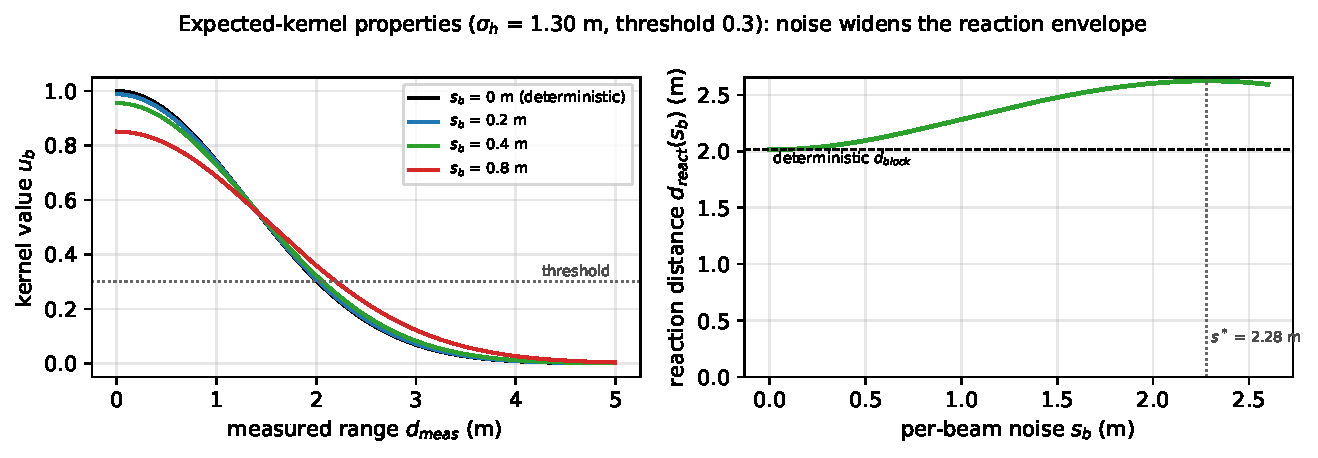
\includegraphics[width=0.92\textwidth]{figures/kernel_theory.pdf}
\caption{The expected kernel for the reference payload. Left: $u_b$ against
measured range for four noise levels; the curves cross at
$d_{\mathrm{meas}} = \sqrt{\sigma_h^2 + s_b^2}$. Right: the reaction
distance of Proposition~2.}
\label{fig:theory}
\end{figure}

\paragraph{Cost.} Per step P-VFH adds, over the deterministic histogram,
one square root and one exponential per beam for $u_b$ (and one error
function per beam for the diagnostic $p_b$): $O(n_{\mathrm{beams}})$ extra
work on top of the $O(n_{\mathrm{beams}} \cdot n_{\mathrm{obstacles}})$
raycast both share. The measured per-step compute is in
Table~\ref{tab:e1}.
Per sector, kernels compose by \textbf{max} --- the nearest-return rule, as in
the deterministic stack (kernels are not probabilities, so noisy-OR would
double-count). The two layers then flow through the same VFH+ propagation,
smoothing, threshold, valley search and hysteresis as
Section~\ref{sec:algorithms}, and the chosen valley direction is fused with
the APF obstacle reflex (computed on the same noisy scan) exactly like the
deterministic composition.

\subsection{The recursive range filter}
\label{sec:rfilter}

What the sensor model buys is knowledge of how much to trust one scan.
P-VFH keeps, for every beam $b$ of the fixed lidar fan, a scalar Bayesian
(Kalman) estimate of the range along that bearing: the true range is
modelled as a random walk with per-step standard deviation $q = 0.08$~m
(sensor and mover motion between two scans), and each scan is a
measurement with the sensor's own $s_b$:
\begin{equation}
K_b = \frac{P_b + q^2}{P_b + q^2 + s_b^2},\qquad
\hat d_b \leftarrow \hat d_b + K_b\,(d_{\mathrm{meas},b} - \hat d_b),\qquad
P_b \leftarrow (1 - K_b)(P_b + q^2).
\label{eq:rfilter}
\end{equation}
The posterior mean $\hat d_b$ and the posterior standard deviation
$\sqrt{P_b} \le s_b$ then replace $d_{\mathrm{meas},b}$ and $s_b$ in the
expected kernel~\eqref{eq:ukernel} and in the reflex. Three points:
\begin{itemize}[leftmargin=1.6em]
\item \textbf{The gain is set by the noise model, not tuned.} For a
precise sensor ($s_b \ll q$) $K_b \to 1$ and nothing is filtered, so the
deterministic limit of Proposition~1 survives; for a noisy one the filter
averages over several scans.
\item \textbf{Discontinuities are not smoothed.} An innovation larger than
three standard deviations (a beam sliding off an edge, a mover entering
the beam) re-initialises that beam to the measurement, so a newly visible
obstacle is never seen late.
\item \textbf{Scope.} The filter needs a fixed beam fan and one persistent
history, so it runs for the transport leader with the lidar; with the
body-fixed ToF fan P-VFH falls back to the single-scan kernel.
\end{itemize}
\code{'pvfh\_filt'} applies the same filter to the deterministic law, so
the grid separates what the filter contributes from what the expected
kernel contributes.

\subsection{The two APF+VFH compositions}

\begin{table}[h]
\centering
\begin{tabular}{@{}lp{6.2cm}p{6.2cm}@{}}
\toprule
 & \textbf{Phase 1 (forming)} & \textbf{Phase 2 (transport)}\\
\midrule
Architecture & \textbf{Cascaded}: APF builds a virtual goal
$\mathbf{g}_v = \mathbf{p} + \mathbf{F}$, VFH steers toward it & 
\textbf{Weighted sum}: $\theta_{\mathrm{raw}}$ from
$w_g\,\hat{\mathbf{v}}_{\mathrm{goal}} + w_v\,\hat{\mathbf{v}}_{\mathrm{vfh}}$\\
APF role & slot attraction + formation-mate repulsion & pure goal attraction
(no mates: the leader has none)\\
VFH margin & robot radius & \textbf{circumradius} $+$ robot radius\\
Speed logic & $v = V_f \min(1, e_i/r_{\mathrm{slow}})$ & $v = V \cdot
\text{speed\_scale}$ (movers)\\
\bottomrule
\end{tabular}
\caption{The same two algorithms, composed differently per phase. In
transport the goal weight is faded by the agreement between the two
directions, $w_g \max(0, \hat{\mathbf{v}}_{\mathrm{goal}} \cdot
\hat{\mathbf{v}}_{\mathrm{steer}})$: with a fixed weight a $90^\circ$ detour
chosen by the steering law is dragged back to $63^\circ$, toward the
obstacle it was avoiding (\code{cfg.blend\_fade}; not applied to
\code{'apf'}).}
\label{tab:arch}
\end{table}

\subsection{Convoy / queueing behaviour (Phase 1 only)}

Robots squeezed by a \emph{compact static} obstacle (largest footprint
$\le 2.0$~m --- pillars and pallets, never walls or shelf racks) may switch to
single-file mode: the group elects a leader, the leader leaves a trail, and
followers target points at $1.0$~m spacing along the trail
(\code{point\_along\_trail\_} \code{\allowbreak behind.m}). This trades
formation geometry for progress through a pinch, then reforms on the other
side. Movers are never convoy anchors --- the trail logic assumes a
stationary thing to queue behind.

\subsection{The safety gate, stuck escape and the anti-deadlock layer}
\label{sec:gate}

\paragraph{Atomic pose commit.} Each transport step proposes a new pose
(position \emph{and} heading). It is committed only if the whole body is
collision-free at $t$ and $t+\Delta t$. If the translation is refused, the
rotation alone is tested (a rigid frame may pivot about its centroid); if
that is refused too, the pose is held; a body held for more than five
steps makes a \emph{recovery move} --- it backs up half a step along its
axis, or turns the other way round --- because a body that can neither
advance nor rotate would otherwise hold forever. Every refusal is logged
as a \emph{gate rejection}. Because the gate uses the exact world geometry, a
committed pose is never in static contact; the rejection count is therefore
the safety metric of this report --- it counts the collisions the steering
law \emph{would} have caused without a supervisor. (Before the audit the
heading was committed without the check, so a blocked body rotated in place
into the obstacle; \S\ref{sec:audit}.) Contact can still occur from the
other side: movers are kinematic and never yield, so a mover can drive into
a body that is holding still. Those steps are counted separately as
\emph{mover contacts}.

\paragraph{Load-carrying motion limits.} The frame is a rigid payload on
$K$ robots, and a slot at distance $r_c$ from the centre moves at up to
$v + \lvert\omega\rvert r_c$. An unconstrained yaw rate therefore asks the
outer robot for speed it does not have: in a reference run without limits
a corner robot needed $3.0$~m/s while the centre drove $0.6$~m/s, with yaw
accelerations up to $13.7$~rad/s$^2$. Each step the commanded turn is
shaped, for every steering law alike: a braking curve
$\lvert\omega\rvert \le 0.8\sqrt{2\,\alpha_{\max}\lvert e_\theta\rvert}$
(never turn faster than can be stopped on the target heading); yaw rate
$\lvert\omega\rvert \le (v_{\max} - v_{\mathrm{floor}})/r_c$; yaw
acceleration $\lvert\dot\omega\rvert \le \alpha_{\max} = 2.5$~rad/s$^2$;
and speed $v \le \min\bigl(v_{\max} - \lvert\omega\rvert r_c,\;
a_{\mathrm{lat}}/\lvert\omega\rvert\bigr)$, with robot speed limit
$v_{\max} = 1.0$~m/s, lateral-acceleration limit
$a_{\mathrm{lat}} = 0.8$~m/s$^2$ and speed floor
$v_{\mathrm{floor}} = 0.5\,V$. The floor matters: a first version let the
yaw rate rise until the speed reached zero, and the formation then pivoted
in place in a mover's lane and was run into. The formation slows down to
turn, but does not stop to pivot unless the safety gate blocks its
translation. \textbf{The limits are off by default} (\code{cfg.kin}) and
evaluated as their own experiment, E14 (\S\ref{sec:e14}): the steering
stack was tuned for the agile body, and switching the limits on without
re-tuning it makes the formation slow enough to be caught by traffic. At the switch from forming to transport the
robots' residual slot error (up to the $0.3$~m forming tolerance) decays
with a $1$~s time constant rather than vanishing in one step.

\paragraph{Escape probe.} When a step is rejected repeatedly (5 consecutive times), the agent probes 36
headings sorted by deviation from the desired one and takes the first along
which the body can actually \emph{translate} one step. Two classic
implementation bugs this avoids: (i) testing the rotated body \emph{in place}
(a body blocked ahead is not itself in collision, so the probe trivially
``succeeds'' without escaping) and (ii) testing only the slot points, which a
0.8~m pillar can sit between undetected.

\paragraph{Anti-deadlock layer.} Two additions close the loop between
probing and going, identically for \emph{every} steering law: (i) a
\emph{progress window} --- $150$ steps ($15$~s) with less than $0.30$~m of
net motion along the start$\to$goal axis forces a probe even when every
step was accepted, catching stalls made of legal micro-steps; (ii)
\emph{commit-after-probe} --- a found escape heading is held for $40$ steps
(rate-limited turn, every pose still gated), and a window-triggered probe
skips headings within $0.5$~rad of the previous escape so it cannot
re-commit to the same dead end. \code{cfg.adl.enable = false} restores the
one-shot probe; E9 (\S\ref{sec:e9}) measures the difference.

\subsection{Feasibility check (run before trusting anything)}

\code{world\_feasibility.m} flood-fills a thresholded clearance grid with
bisection on the threshold to find the corridor bottleneck --- the widest
half-corridor on the best start$\to$goal path. A rigid $2\times2$ block at
spacing $s$ needs circumradius
$c = (N-1)\,s\,\sqrt{2}/2 + r$; if $c$ exceeds the bottleneck, \emph{no}
controller tuning will get the formation through, and the script either
auto-reduces $s$ or fails loudly. For the dynamic world: bottleneck
$1.22$~m, spacing used $1.18$~m, circumradius $1.01$~m, margin $0.21$~m.
